% Autor: Leonhard Segger, Alexander Neuwirth
% Datum: 2017-10-30
\documentclass[
	% Papierformat
	a4paper,
	% Schriftgröße (beliebige Größen mit „fontsize=Xpt“)
	12pt,
	% Schreibt die Papiergröße korrekt ins Ausgabedokument
	pagesize,
	% Sprache für z.B. Babel
	ngerman
]{scrartcl}

% Achtung: Die Reihenfolge der Pakete kann (leider) wichtig sein!
% Insbesondere sollten (so wie hier) babel, fontenc und inputenc (in dieser
% Reihenfolge) als Erstes und hyperref und cleveref (Reihenfolge auch hier
% beachten) als Letztes geladen werden!

% Silbentrennung etc.; Sprache wird durch Option bei \documentclass festgelegt
\usepackage{babel}
% Verwendung der Zeichentabelle T1 (Sonderzeichen etc.)
\usepackage[T1]{fontenc}
% Legt die Zeichenkodierung der Eingabedatei fest, z.B. UTF-8
\usepackage[utf8]{inputenc}
% Schriftart
\usepackage{lmodern}
% Zusätzliche Sonderzeichen
\usepackage{textcomp}

% Mathepaket (intlimits: Grenzen über/unter Integralzeichen)
\usepackage[intlimits]{amsmath}
% Ermöglicht die Nutzung von \SI{Zahl}{Einheit} u.a.
\usepackage{siunitx}
% Zum flexiblen Einbinden von Grafiken (\includegraphics)
\usepackage{graphicx}
% Abbildungen im Fließtext
\usepackage{wrapfig}
% Abbildungen nebeneinander (subfigure, subtable)
\usepackage{subcaption}
% Funktionen für Anführungszeichen
\usepackage{csquotes}
% Zitieren, Bibliographie
\usepackage{biblatex}


% Zur Darstellung von Webadressen
\usepackage{url}
%chemische Formeln
\usepackage[version=4]{mhchem}
% siunitx: Deutsche Ausgabe, Messfehler getrennt mit ± ausgeben
\usepackage{floatrow}
\floatsetup[table]{capposition=top}
\usepackage{float}
% Verlinkt Textstellen im PDF-Dokument
\usepackage[unicode]{hyperref}
% "Schlaue" Referenzen (nach hyperref laden!)
\usepackage{cleveref}
\sisetup{
	locale=DE,
	separate-uncertainty
}
\bibliography{14Mo_A2_30-04-2018_References}

\begin{document}
	
	\begin{titlepage}
		\centering
		{\scshape\LARGE Versuchsbericht zu \par}
		\vspace{1cm}
		{\scshape\huge A2 - Franck-Hertz-Versuch \par} 
		\vspace{2.5cm}
		{\LARGE Gruppe 14Mo \par}
		\vspace{0.5cm}
		
		{\large Alexander Neuwirth (E-Mail: a\_neuw01@wwu.de) \par}
		{\large Leonhard Segger (E-Mail: l\_segg03@uni-muenster.de) \par}
		\vfill
		
		durchgeführt am 30.04.2018\par
		betreut von\par
		{\large Fabian Schöttke}
		
		\vfill
		
		{\large \today\par}
	\end{titlepage}
	\tableofcontents
	\newpage

	%TODO mehr TODO in Default	

	\section{Kurzfassung}
	%TODO Hypothese	und deren Ergebnis
	%TODO Ergebnisse, auch Zahlen, mindestens wenn's halbwegs Sinn ergibt
	%TODO Was wurde gemacht
	
	\section{Methoden}
	Untersucht wurde eine Franck-Hertz-Röhre mit Quecksilberfüllung und eine mit Neonfüllung.
	Diese wurden, wie in  \cref{Roehren_Schaltung} dargestellt, verschaltet. %ist das schön?
	Die Quecksilberröhre befand sich in einem Ofen, der sie auf bis zu \SI{300}{\degreeCelsius} aufheizen kann.
	Der Anodenstrom ist sehr klein, weshalb er vom Betriebsgerät in eine Spannung $U_A$ umgewandelt wurde, die zum Anodenstrom proportional ist.
	
	Zunächst wurde die $I_A/U_B$-Charakteristik der Röhre mit Quecksilberfüllung bei Zimmertemperatur aufgenommen.
	Dazu wurde die Beschleunigungsspannung $U_B$ langsam erhöht und diese sowie die Spannung $U_A$ gemessen.
	
	Im Anschluss wurde der Ofen auf ca. \SI{180}{\degreeCelsius} erhitzt.
	Dann wurde das Betriebsgerät so eingestellt, dass es eine Dreieckspannung mit einer Frequenz von \SI{60}{\hertz} als Beschleunigungsspannung ausgibt.
	Der resultierende Anodenstrom wurde zunächst mit einem Oszilloskop betrachtet und Bremsspannung $U_B$ und Heizstrom $I_H$ so eingestellt, dass sich mindestens drei Minima der Franck-Hertz-Kurve ablesen ließen.
	Dann wurde mithilfe manueller Reglung der Beschleunigungsspannung die $I_A/U_B$-Charakteristik wie zuvor aufgenommen und die Temperatur im Ofen gemessen.
	
	Analog wurde die Neon-Röhre bei Raumtemperatur untersucht, wobei hier zusätzlich ein Steuergitter (mit Spannung $U_S$) verwendet wurde, um störende Einflüsse durch Abstoßung der Elektronen untereinander zu verringern. %TODO Ist das so korrekt?
	
	\begin{figure}[H]
		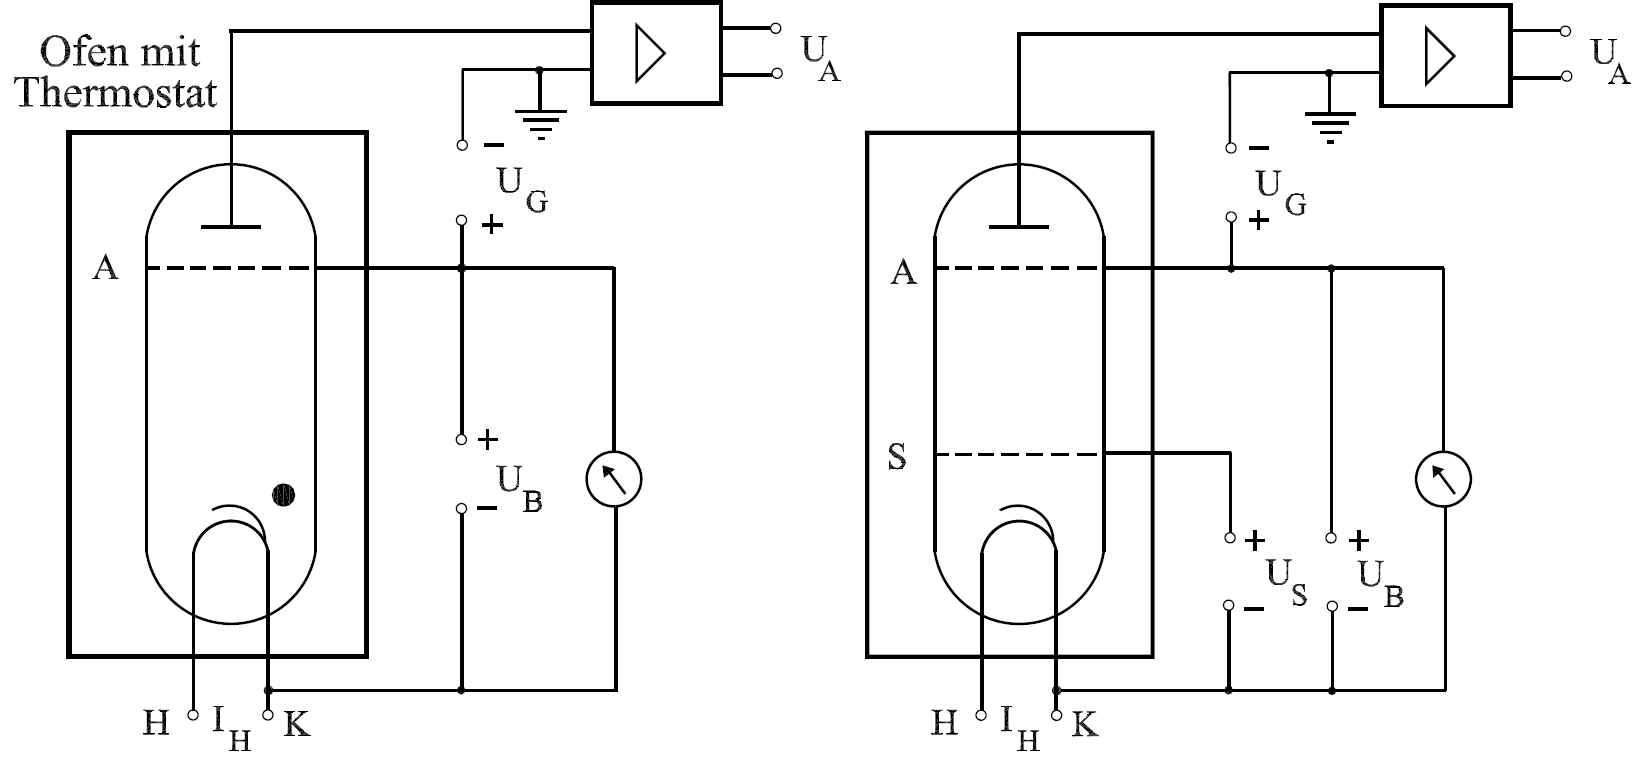
\includegraphics[width=0.7\textwidth]{Roehren}
		\centering
		\caption{Schaltungen der Franck-Hertz-Röhren mit Quecksilber (links) und Neon (rechts).\cite{Roehren} }
		\label{Roehren_Schaltung}
		\centering
	\end{figure}

	\section{Ergebnisse und Diskussion}
	%TODO Datenanalyse -> Überschrift?
	%TODO Unsicherheiten
	

	\subsection{Beobachtung}
	%TODO Komplikationen mit MEssgerät => Trioden linie graph => ist Falsch 
	
	%TODO Mann misst auch eine Spannung selbst wenn keine Beschleunigungs spannung angelegt ist
	
	%TODO Temperatur schwankte zwischen 165 und 180
	%TODO Oszi graphen (ggf. nur der eine)
	%TODO Erhöhung von Gegenspannung => Ausgangsspannung kleiner
	%TODO T > 190°C Verlauf => MAxima "fallen runter" ((=> kein durchkommen der e- mehr))
	%TODO Beim Neon sieht man leuchtende Linien (zuerst eine dann mehrere zusätzlich).
	%TODO Bem HG ist kein Leuchten zusehen
	%TODO Sichtbare Charakteristik /= Messungscharakteristik
	
	%TODO Gegenspannung s wert erwähnen
	
	\begin{figure}[H]
		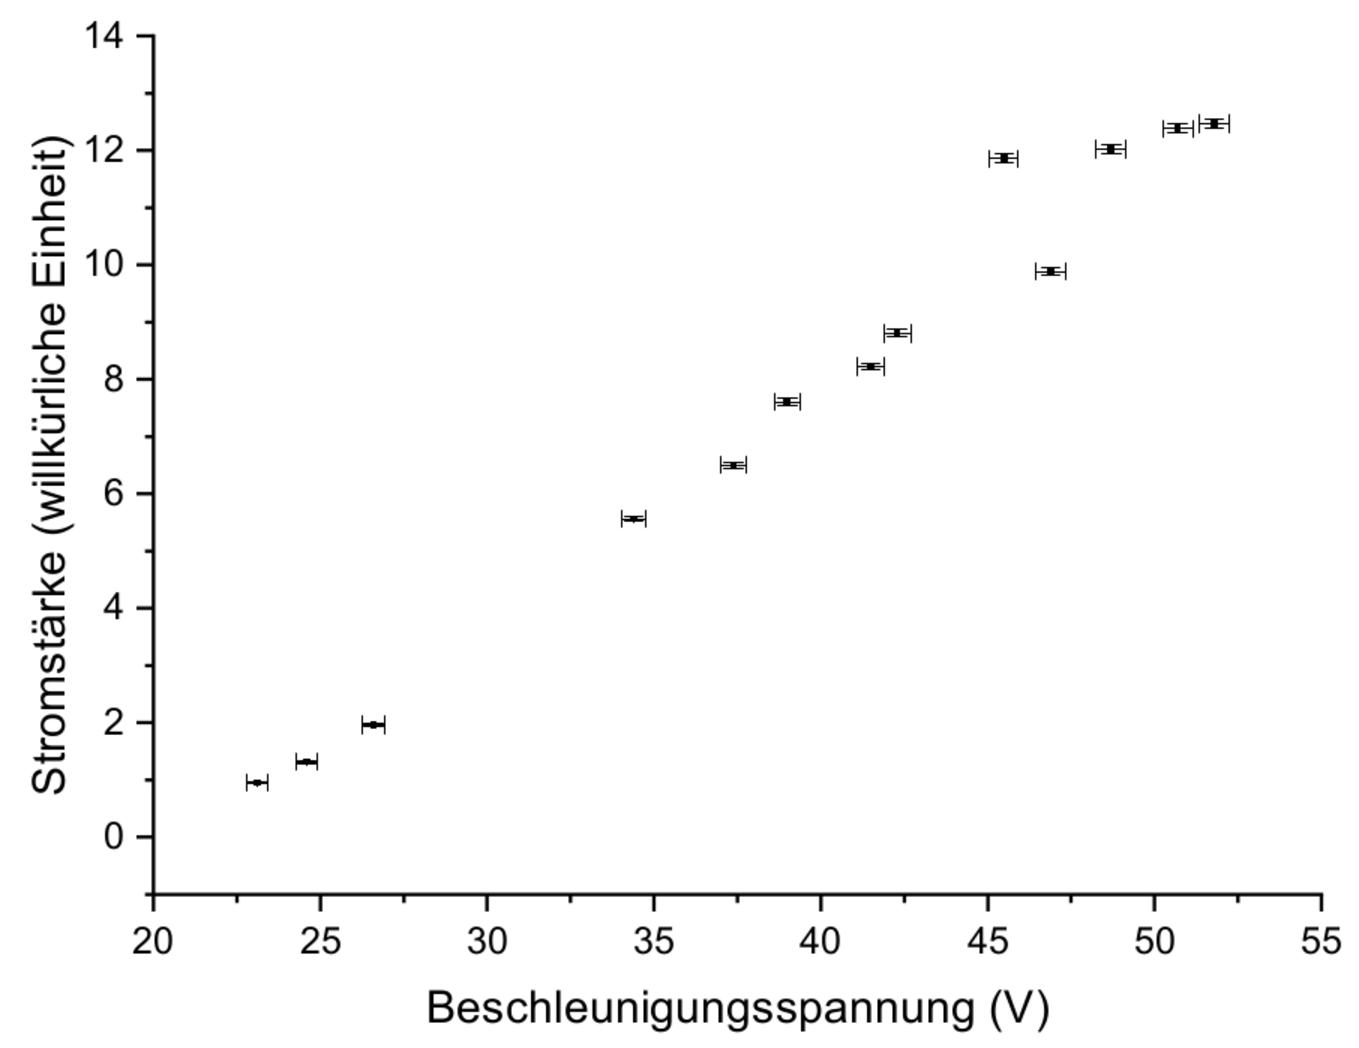
\includegraphics[width=0.7\textwidth]{Hg19}
		\centering
		\caption{Aufgenommene Quecksilber-Charakteristik bei $T$=$\SI{19,0 +- 1,5}{\degreeCelsius}$. Die Stromstärke wurde mit einem Operationsverstärker in eine messbare Spannung umgewandelt.}
		\label{Hg19}
		\centering
	\end{figure}
	
	\subsection{Datenanalyse}
	\subsubsection{Unsicherheiten}
	Die Unsicherheit des  Voltmeters beträgt $\pm (0,5\% + \SI{200}{mV})$ für die Beschleunigungsspannung und $\pm (0,5\% + \SI{20}{mV})$ für die gemessene Spannung (0,5\% vom angezeigten Wert).\cite{FH-Pforzheim} Die zusätzliche Unsicherheit des Operationsverstärkers wird als demgegenüber vernachlässigbar angenommen. 
	
	Die Unsicherheit des Thermometers vom Typ K ist \SI{1,5}{\degreeCelsius} in dem gemessenen Temperaturinterval.\cite{DIN} 
	Zusätzlich ist die Temperatur nicht überall im Heizkasten gleich und schwankte beim Aufnehmen der Quecksilber-Charakteristik von 165 bis \SI{180}{\degreeCelsius}, deshalb wählen wir für diese Messung die Unsicherheit als \SI{7}{\degreeCelsius}.
	
	Bei der Bestimmung der Beschleunigungsspannung an Extremstellen nehmen wir die Unsicherheit als aus dem Verlauf der Kurve und dem Abstand zum nächsten Messpunkt zusammengesetzt an.
	
	\subsubsection{Quecksilber-Charakteristik}
	In \cref{Hg175} ist die $I_A/U_B$-Charakteristik des Quecksilbers bei $T$=$\SI{175 +- 7}{\degreeCelsius}$ dargestellt. Daraus lassen sich folgende Abstände ablesen:
	\begin{itemize}
		\item Maxima:
		\begin{equation*}
			\Delta{U}_1 = \SI{27,1 +- 0,3}{V} -\SI{21 +- 0,1}{V} = \SI{6,1 +- 0,3}{V}
		\end{equation*}
		\item Minima
		\begin{equation*}\Delta{U}_2 = \SI{29,4 +- 0,2}{V} -\SI{24,1 +- 0,2}{V} = \SI{5,3 +- 0,3}{V}\end{equation*}
		\begin{equation*}\Delta{U}_3 = \SI{24,1 +- 0,2}{V}- \SI{18,0 +- 0,5}{V} = \SI{6,1 +- 0,5}{V}\end{equation*}
	\end{itemize}
	Im Mittel ergibt sich ein $\Delta{U_\text{Hg}}$ von $\SI{5,8 +- 0,2}{V}$.
	
	\begin{figure}[H]
		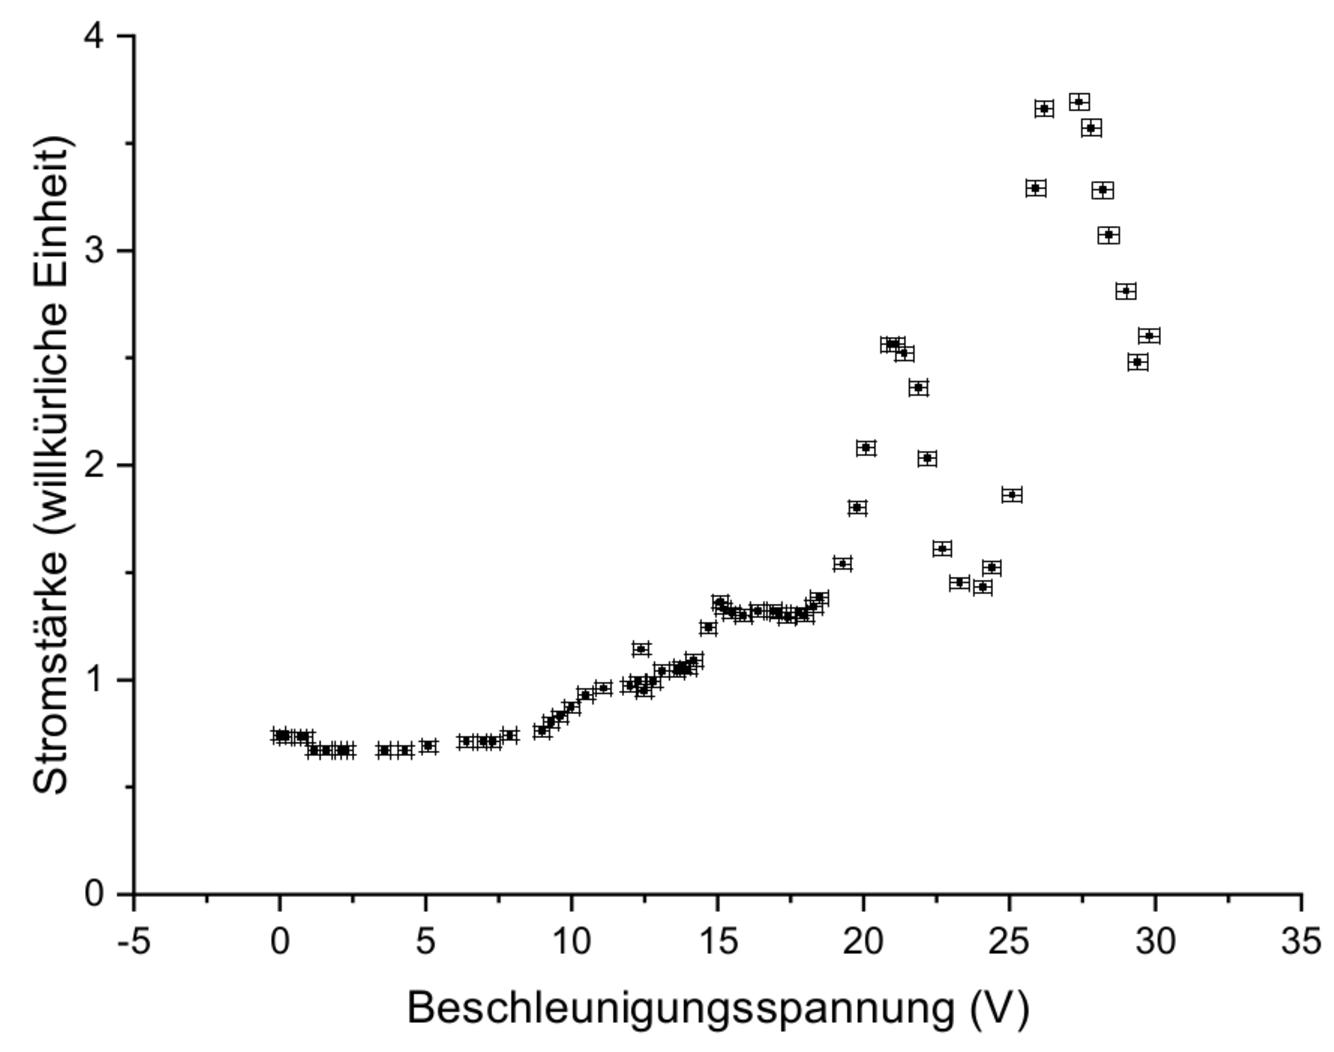
\includegraphics[width=0.7\textwidth]{Hg175}
		\centering
		\caption{Aufgenommene Quecksilber-Charakteristik bei $T$=$\SI{175 +- 7}{\degreeCelsius}$. Die Stromstärke wurde mit einem Operationsverstärker in eine messbare Spannung umgewandelt.}
		\label{Hg175}
		\centering
	\end{figure}


	\subsubsection{Neon-Charakteristik}
	In \cref{Ne19} ist die $I_A/U_B$-Charakteristik des Neons bei $T$=$\SI{19 +- 1,5}{\degreeCelsius}$ dargestellt. Daraus lassen sich folgende Abstände ablesen:
	\begin{itemize}
		\item Maxima:
		\begin{equation*}
		\Delta{U}_1 = \SI{38,8 +- 0,2}{V} -\SI{20,8 +- 0,4}{V} = \SI{18,0+- 0,4}{V}
		\end{equation*}
		\begin{equation*}
		\Delta{U}_2 = \SI{57,2 +- 0,2}{V} - \SI{38,8 +- 0,2}{V} = \SI{18,4 +- 0,3}{V}
		\end{equation*}
		\item Minima
		\begin{equation*}\Delta{U}_3 = \SI{44,9 +- 0,5}{V} -\SI{27,5 +- 0,3}{V} = \SI{17,4 +- 0,6}{V}\end{equation*}
		\begin{equation*}\Delta{U}_4 = \SI{62,9 +- 0,5}{V}- \SI{45,5 +- 0,4}{V} = \SI{18,0 +- 0,7}{V}\end{equation*}
	\end{itemize}
	Im Mittel ergibt sich ein $\Delta{U_\text{Ne}}$ von $\SI{17,9 +- 0,3}{V}$.
	\begin{figure}[H]
		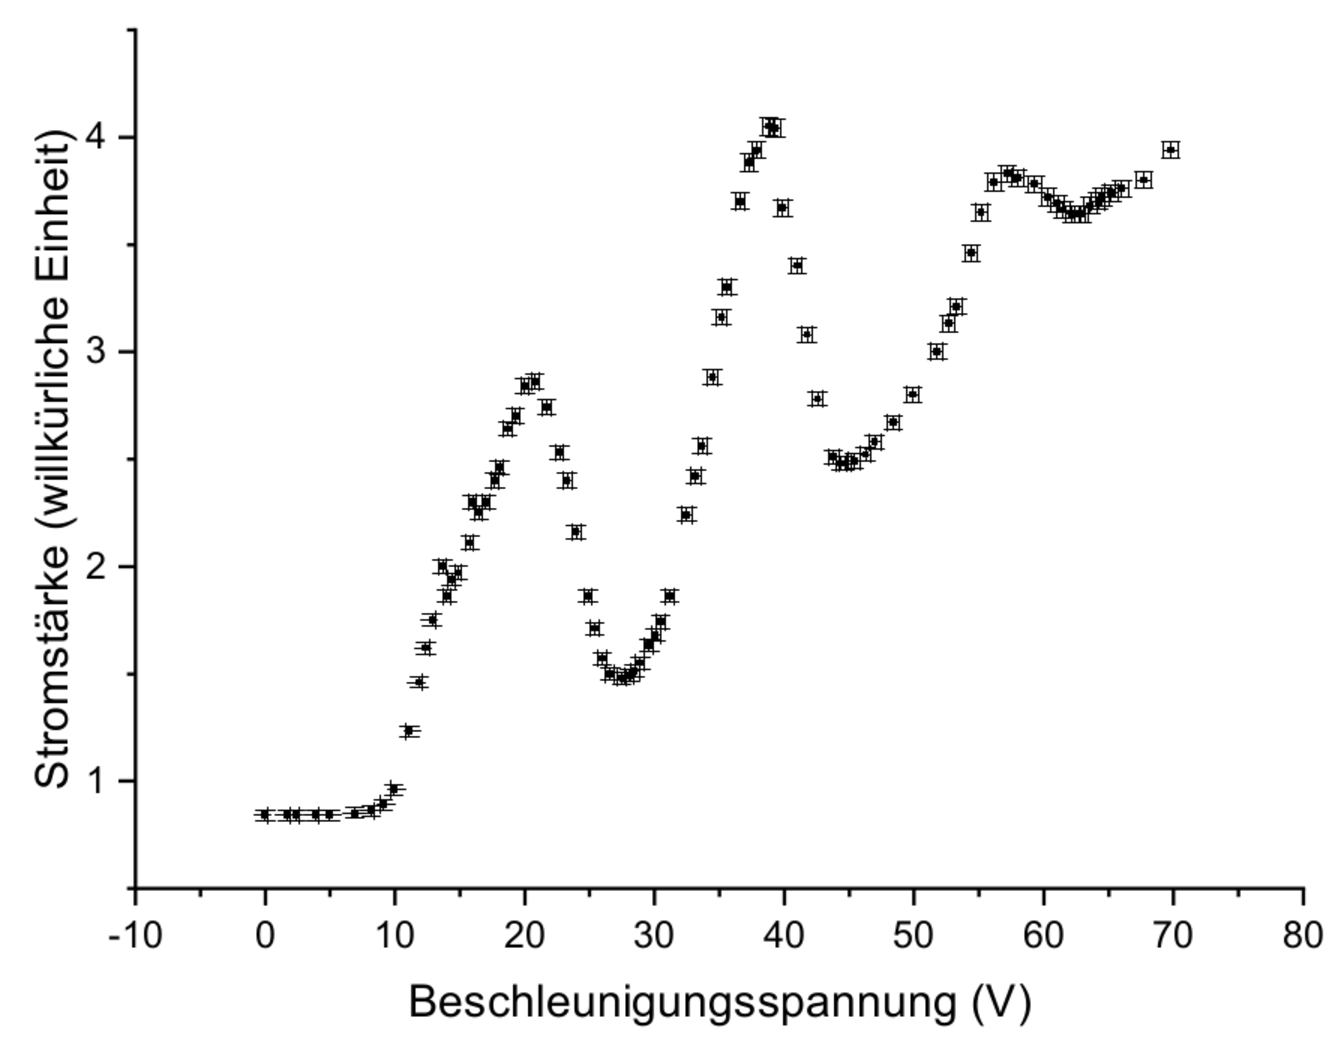
\includegraphics[width=0.7\textwidth]{Ne19}
		\centering
		\caption{Aufgenommene Neon-Charakteristik bei $T$=$\SI{19,0 +- 1,5}{\degreeCelsius}$. Die Stromstärke wurde mit einem Operationsverstärker in eine messbare Spannung umgewandelt.}
		\label{Ne19}
		\centering
	\end{figure}

	\subsubsection{Bestimmen von Anregungsenergie, Wellenlänge und Frequenz der Strahlung}
	Aus den Spannungen lässt sich die kinetische Energie eines Elektrons bestimmen, die nowendig ist um den Resonanzzustand des Atoms anzuregen.
	Sie beträgt $\Delta{E}=\Delta{U}e$.
	Die Frequenz folgt aus $\nu=\Delta{E}/h$ und die Wellenlänge aus $\lambda=c/\nu$.\cite{NIST}
	Die jeweiligen Werte sind in \cref{TabelleEnergie} aufgelistet.
	\begin{table}[H]
		\centering
		\begin{tabular}{ c | c | c | c | c }
			&$\Delta{U}$ & $\Delta{E}$ &  $\nu$ & $\lambda$ \\ \hline
			Quecksilber&\SI{5,8 +- 0,2}{V} &\SI{5,8 +- 0,2}{eV} & \SI{1402 +- 48}{THz} & \SI{214,0 +- 6,3}{nm} \\
			Neon&\SI{17,9+- 0,3}{V} & \SI{17,9+- 0,3}{eV} & \SI{4328 +- 73}{THz} & \SI{69,3 +- 1,2}{nm} \\
		\end{tabular}
		\caption{Aus den Charakteristiken von Quecksilber und Neon berechnete kinetische Energie, sowie  Frequenz und Wellenlänge des emittierten Lichts.}
		\label{TabelleEnergie} 
	\end{table}
	
	\subsubsection{Berechnen der  mittleren freien Weglänge der Elektronen}
	In der Einführung wurde folgende Formel aufgeführt zum Bestimmen der freien Weglänge $\lambda$ der Elektronen:
	\begin{equation}
		\lambda = \frac{k_B T}{\sigma p} \quad \text{mit} \quad \sigma = \pi r_\text{Hg}^2
		\label{frei}
	\end{equation}
	Der Druck $p$ wird durch die Clausius-Clapeyron-Gleichung in integrierter Form bestimmt:
	\begin{equation}
		\ln\left(\frac{p_2}{p_1}\right) = \frac{\Delta{H_\text{m,v}}}{R} \left( \frac{1}{T_1} - \frac{1}{T_2} \right)
		\label{Clausius}
	\end{equation}
	Dabei beträgt die allgemeine Gaskonstante $R$ = $\SI{8,3145}{J/mol/K}$, Verdampfungsenthalpie von Quecksilber $\Delta{H_\text{m,v}}$ =  $\SI{59,3}{kJ/mol}$, Radius eines Quecksilberatoms $r_\text{Hg}$ = $\SI{150}{pm}$ und der Referenzpunkt ist $T_1$ = $\SI{293,15}{K}$ mit $p_1$ = $\SI{0,242}{Pa}$.\cite{Quecksilber}\cite{Enthalpie}\cite{NIST}
	
	Durch Umformen von \cref{Clausius} ergibt sich $p_\text{kalt}$ und $p_\text{warm}$.
	Daraus widerum folgt mit \cref{frei} $\lambda_\text{kalt}$ und $\lambda_\text{warm}$.
	Die so bestimmten Werte sind in \cref{TabelleFrei} enthalten.
	
	\begin{table}[H]
		\centering
		\begin{tabular}{ c | c | c | c }
			&$T$ & $p$ &  $\lambda$ \\ \hline
			kalt&\SI{292.15 +- 1,5}{K} &\SI{0,223+-0,028}{Pa} &  \SI{0,256+- 0,032}{m} \\
			warm&\SI{453.15+- 7}{K} & \SI{1,3+-0,2}{kPa} & \SI{0,068 +- 0,010}{mm} \\
		\end{tabular}
		\caption{Mittlere frei Weglänge von Elektronen in Quecksilberdampf bei Raumtemperatur(kalt) und Heiztemperatur(warm).}
		\label{TabelleFrei} 
	\end{table}
	
	%TODO ANhang mit   Formeln vong GUM???????????????????????????????????!!!!!!!!!!!!???????????????
	
	
	\subsection{Diskussion}
	%TODO Bezug/Nutzten oder sonst was
	%TODO auch hier die Hypothese wiederholen
	
	

	%TODO Bei 0V Beschleunigungsspannung ggf. grundSpannugn am Operationsverstärker /= Null
	%TODO ^^^^^^ bzw bei U_b < U_g
	
	%TODO WARUM ist Ne Licht sichtbar
	
	%TODO Messung /= sichtbarem Ne, da andere Wellenlänge sichtbar vs MEssung
	
	
	%TODO WARUM verschwinden HG Charakteristiken bei T >190°C
	
	%TODO Spannung zu hoch => interne Verlusste müssen ausgeglichen werden?
	%TODO ^^^^^^^Quantisierte Energie denoch deutlich erkennbar
	
	%TODO Weglängen vergleich
	
	\section{Schlussfolgerung}
	%TODO Rückgriff auf Hypothese und drittes Nennen dieser
	
	%TODO Quellen zitieren, Websiten mit Zugriffsdatum
	%TODO Verweise auf das Laborbuch (sind erlaubt)
	%TODO Tabelle + Bilder mit Beschriftung
	\printbibliography
\end{document}
